\begin{code}
  module horst where
\end{code}

The \spx hypertree \hyper is not used to sign the actual messages but the 
public keys of \fors instances which in turn are used to sign message digests. 
\fors (pronounced [\textipa{fO:rs}]), short for forest of random subsets, is a few-time 
signature scheme (FTS). \fors is an improvement of \horst~\cite{Bernstein2015} 
which in turn is a variant of \hors~\cite{Reyzin2002}. 
For security it is essential that the input to \fors is the output of a
hash function. In the following we describe \fors as acting on bit strings.


\fors uses parameters $k$ and $t=2^a$ (example parameters are $t=2^{15}, k=10$). 
\fors signs strings of length $ka$ bits. Here, we deviate from defining 
sizes in bytes as the message length in bits might not be a multiple of eight.
The private key consists of $kt$ 
random $n$-byte strings grouped
into $k$ sets, each containing $t$ $n$-byte strings. The private key values
are pseudorandomly generated from the main private seed \sseed in the \spx private
key. In \spx, the \fors private key values are only temporarily generated as an 
intermediate result when computing the public key or a signature. 

The \fors public key is a single $n$-byte hash value. It is computed as the 
tweakable hash of the root nodes of $k$ binary hash trees. Each of these binary 
hash trees has height $a$ and is used to authenticate the $t$ private key
values of one of the $k$ sets. Accordingly, the leaves of a tree are the 
(tweakable) hashes of the values in its private key set.

A signature on a string $M$ consists of $k$ private key values -- one per 
set of private key elements -- and the 
associated authentication paths. To compute the signature, \md is 
split into $k$ $a$-bit strings. As \md is a sequence of bytes,
we first convert to a bit-string by enumerating the bytes in \md,
internally enumerating the bits within a byte from least to most significant.
Next, each of these bit strings is 
interpreted as an integer between $0$ and $t-1$. Each of these integers is used to
select one private key value from a set. I.e., if the first integer is $i$, the
$i$th private key element of the first set gets selected and so on. The signature
consists of the selected private key elements and the associated authentication 
paths.

\spx uses implicit verification for \fors, only using a method to compute
a candidate public key from a signature. This is done by computing root nodes 
of the $k$ trees using the indices computed from the input string as well as 
the private key values and authentication paths form the signature. The 
tweakable hash of these roots is then returned as candidate public key.

%
We now describe the parameters and algorithms for \fors.

\subsection{\fors Parameters}\label{sec:fors:params}
\fors uses the parameters $n$, $k$, and $t$; they all take positive integer 
values.
These parameters are summarized as follows:
\begin{itemize}
  \item $n$: the security parameter; it is the length of a private key, public 
  key, or signature element in bytes. 
  \item $k$: the number of private key sets, trees and indices computed 
  from the input string.
  \item $t$: the number of elements per private key set, number of leaves per 
  hash tree and upper bound on the index values. The parameter $t$ MUST 
  be a power of $2$. If $t = 2^a$, then the trees have height $a$ and the 
  input string is split into bit strings of length $a$.
\end{itemize}
Inputs to \fors are bit strings of length $k\log t$.

\begin{figure}[htb]
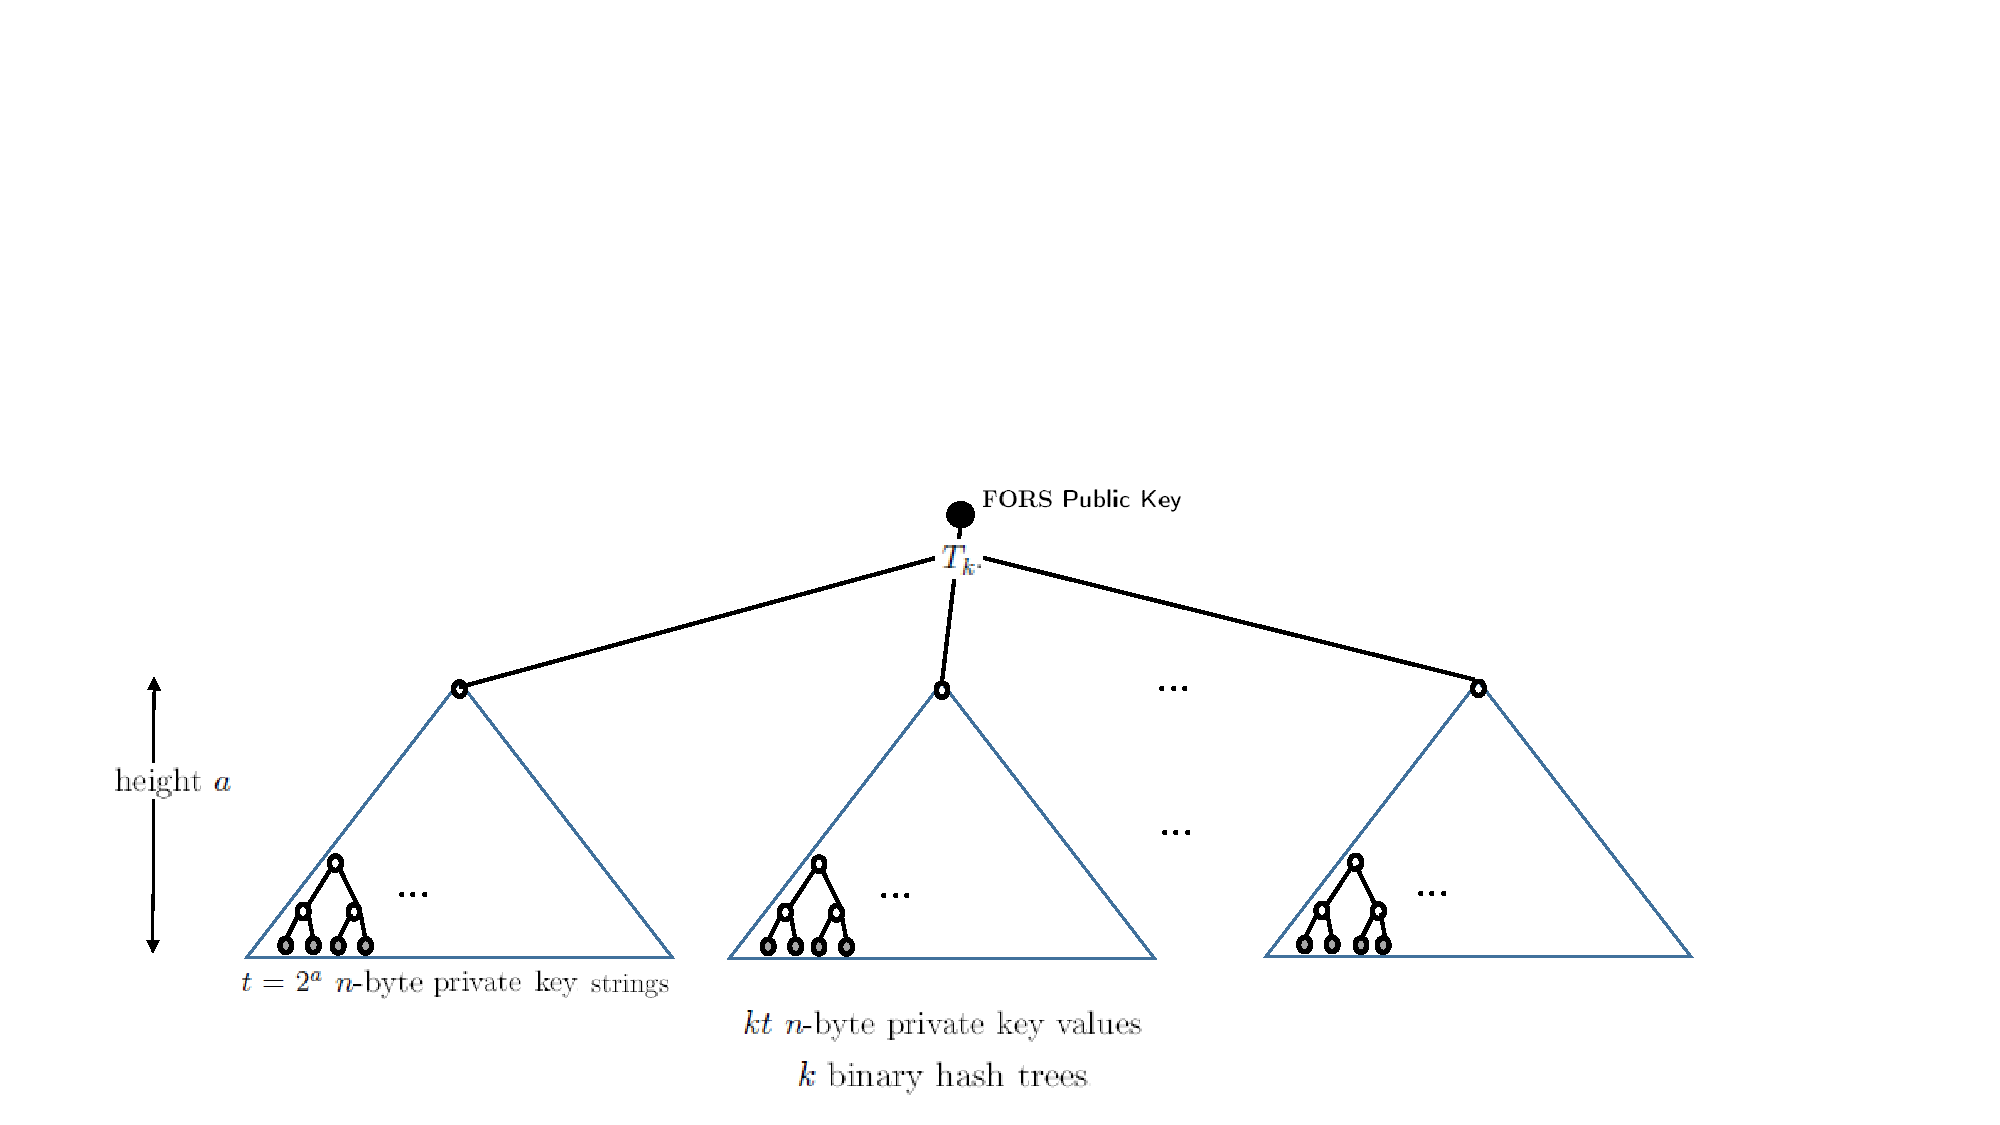
\includegraphics[width=7in,trim={0.5cm 0.5cm 0.5cm 7cm}, clip]{pics/fors_tree.pdf}
\caption{FORS trees and PK}
\end{figure}

\subsection{\fors Private Key (Function \texttt{fors\_SKgen})} 
In the context of \spx, a \fors private key is the single private seed \sseed
contained in the \spx private key. It is used to generate the $kt$ $n$-byte 
private key values using \sphincsPRF with a \fors key generation address. While these values are 
logically grouped into a two-dimensional array, for implementations it makes sense to assume they 
are in a one-dimensional array of length $kt$. 
The $j$th element of the $i$th set is then stored at $\sk[it + j]$. 
To generate one of these elements, a \fors key generation address \skadrs is used, that encodes the 
position of the \fors key pair within \spx and has 
tree height set to $0$ and leaf index set to $it+j$: 

\begin{lstlisting}[label=alg:fors_skgen, language=pseudoc,
                   caption=\texttt{fors\_SKgen} -- Computing a \fors private key value.]
#Input: secret seed SK.seed, address ADRS, secret key index idx = it+j
#Output: FORS private key sk

fors_SKgen(SK.seed, ADRS, idx) {
  skADRS = ADRS; // copy address to create key generation address
  skADRS.setType(FORS_PRF);
  skADRS.setKeyPairAddress(ADRS.getKeyPairAddress());
  
  skADRS.setTreeHeight(0);
  skADRS.setTreeIndex(idx);
  sk = PRF(SK.seed, skADRS);

  return sk;
}
\end{lstlisting}

\subsection{\fors TreeHash (Function \forstreehash)}
   Before coming to the \fors public key, we have to discuss computation of the 
   trees.
   For the computation of the $n$-byte nodes in the \fors hash trees,
   the subroutine \forstreehash is used. It is essentially the same algorithm
   as \treehash (\autoref{algo:treehash}) in \autoref{sec:xmss}. The two 
   differences are how the leaf nodes are computed and how addresses are handled.
   However, as the addresses are similar, an implementation can implement both
   algorithms in the same routine easily.
   
   Algorithm \forstreehash accepts a secret seed \sseed,
   a public seed \pseed, an unsigned integer $s$ (the start index), an
   unsigned integer $z$ (the target node height), and an address \adrs that
   encodes the address of the \fors key pair. As for \treehash, the
   \forstreehash algorithm returns the root node of a tree of height $z$ with
   the leftmost leaf being the hash of the private key element at index $s$. 
   Here, $s$ is ranging over the whole $kt$ private key elements.
   It is REQUIRED that $s\ \%\ 2^z = 0$, i.e. that the leaf at index $s$ is a
   leftmost leaf of a sub-tree of height $z$.  Otherwise the algorithm fails
   as it would compute non-existent nodes.  
   
   \begin{lstlisting}[breaklines=true, label=algo:forstreehash, language=pseudoc,
                   caption=The \forstreehash algorithm.]

# Input: Secret seed SK.seed, start index s, target node height z, public seed PK.seed, address ADRS
# Output: n-byte root node - top node on Stack

fors_treehash(SK.seed, s, z, PK.seed, ADRS) {
     if( s % (1 << z) != 0 ) return -1;
     for ( i = 0; i < 2^z; i++ ) {
       sk = fors_SKgen(SK.seed, ADRS, s+i) 
       node = F(PK.seed, ADRS, sk);
       ADRS.setTreeHeight(1);
       ADRS.setTreeIndex(s + i);
       while ( Top node on Stack has same height as node ) {
          ADRS.setTreeIndex((ADRS.getTreeIndex() - 1) / 2);
          node = H(PK.seed, ADRS, (Stack.pop() || node));
          ADRS.setTreeHeight(ADRS.getTreeHeight() + 1);
       }
       Stack.push(node);
     }
     return Stack.pop();
}

\end{lstlisting}

\subsection{\fors Public Key (Function \forspkgen)}
In the context of \spx, the \fors public key is never generated alone. It is 
only generated together with a signature. We include \forspkgen
for completeness, a better understanding, and testing. Algorithm \forspkgen takes 
a private seed \sseed, a public seed \pseed, and a \fors address \adrs. The 
latter encodes the position of the \fors instance within \spx. It outputs a 
\fors public key.

\begin{lstlisting}[label=alg:fors:pkgen, language=pseudoc,
                   caption=\forspkgen\ -- Generate a FORS public key.]

# Input: Secret seed SK.seed, public seed PK.seed, address ADRS
# Output: FORS public key PK

fors_PKgen(SK.seed, PK.seed, ADRS) {
     forspkADRS = ADRS; // copy address to create FTS public key address

     for(i = 0; i < k; i++){
         root[i] = fors_treehash(SK.seed, i*t, a, PK.seed, ADRS);
     }
     forspkADRS.setType(FORS_ROOTS);
     forspkADRS.setKeyPairAddress(ADRS.getKeyPairAddress());
     pk = T_k(PK.seed, forspkADRS, root);
     return pk;
}
\end{lstlisting}

\subsection{\fors Signature Generation (Function \forssign)}
A \fors signature is a length $k(\log t + 1)$ array of $n$-byte strings. It contains 
$k$ private key values, $n$-bytes each, and their associated authentication
paths, $\log t$ $n$-byte values each.

The algorithm \forssign takes a $(k\log t)$-bit string $M$, a private seed \sseed, 
a public seed \pseed, and an address \adrs. The latter encodes the position of 
the \fors instance within \spx. It outputs a \fors signature \forssig.

\begin{lstlisting}[label=alg:fors_sign, language=pseudoc,
                   caption=\forssign\ -- Generating a FORS signature on string $M$.]
#Input: Bit string M, secret seed SK.seed, address ADRS, public seed PK.seed
#Output: FORS signature SIG_FORS

fors_sign(M, SK.seed, PK.seed, ADRS) {  
  // compute signature elements 
  for(i = 0; i < k; i++){
    // get next index
    unsigned int idx = bits i*log(t) to (i+1)*log(t) - 1 of M;
    
    // pick private key element
    SIG_FORS = SIG_FORS || fors_SKgen(SK.seed, ADRS, i*t + idx) ;
    
    // compute auth path
    for ( j = 0; j < a; j++ ) {
      s = floor(idx / (2^j)) XOR 1;
      AUTH[j] = fors_treehash(SK.seed, i * t + s * 2^j, j, PK.seed, ADRS);
    } 
    SIG_FORS = SIG_FORS || AUTH;
  }
  return SIG_FORS;
}
\end{lstlisting}

The data format for a signature is given in \autoref{fig:fors:sig}.

\begin{figure} [h]
  \begin{center}
    \begin{tabular}{|c|}
      \hline
      \\[-0.5em] Private key value (tree 0) ($n$ bytes) \\[-0.5em] \\ \hline
      \\[-0.5em] \auth (tree 0) ($\log t\cdot n$ bytes) \\[-0.5em] \\ \hline
      \\[-0.5em] ... \\[-0.5em] \\ \hline
      \\[-0.5em] Private key value (tree $k-1$) ($n$ bytes) \\[-0.5em] \\ \hline
      \\[-0.5em] \auth (tree $k-1$) ($\log t\cdot n$ bytes) \\[-0.5em] \\ \hline
    \end{tabular}
  \end{center}
  \caption{\fors signature}
  \label{fig:fors:sig}
\end{figure}

\subsection{\fors Compute Public Key from Signature (Function \forspkfromsig)}

   \spx makes use of implicit signature verification of \fors signatures. 
   A \fors signature is used to compute a candidate \fors public key. This 
   public key is used in further computations (message for the signature of 
   the \xmss tree above) and implicitly verified by the outcome of that computation. Hence, this specification does 
   not contain a \texttt{fors\_verify} method but the method 
   \forspkfromsig. 
   
   The method \forspkfromsig takes a $k\log t$-bit string \msg, 
   a \fors signature \forssig, a public seed \pseed, and 
   an address \adrs. The latter encodes the position of the \fors 
   instance within the virtual structure of the \spx key pair. 
   First, the roots of the $k$ binary hash trees are computed using 
   \forstreehash. Afterwards the roots are hashed using the tweakable hash
   function $\sphincsT_k$.
%    \TODO {Clarify that this step takes place by the signer. --Andy: No, it takes place at signer AND verifier. On the signer side it is kind of a misuse of this method.}
   The algorithm \forspkfromsig is given 
   as \autoref{alg:fors:rootFromSig}. The method \forspkfromsig makes use of 
   functions $\forssig\texttt{.getSK(i)}$ and $\forssig\texttt{.getAUTH(i)}$. The 
   former returns the $i$th secret key element stored in the 
   signature, the latter returns the $i$th authentication path stored in
   the signature.
%    \TODO{Looks like what is missing here is that you calculate the FORS PK and compare it to the 
%    PK extracted with \forspkfromsig. --Andy: No, that's exactly what implicit signature verification is about. }
   
   
   
\begin{lstlisting}[breaklines=true, label=alg:fors:rootFromSig, language=pseudoc,
                   caption=\forspkfromsig\ -- 
                   Compute a \fors public key from a \fors signature.]

# Input: FORS signature SIG_FORS, (k lg t)-bit string M, public seed PK.seed, address ADRS
# Output: FORS public key

fors_pkFromSig(SIG_FORS, M, PK.seed, ADRS){
     
  // compute roots
  for(i = 0; i < k; i++){
    // get next index
    unsigned int idx = bits i*log(t) to (i+1)*log(t) - 1 of M;
    
    // compute leaf
    sk = SIG_FORS.getSK(i);
    ADRS.setTreeHeight(0);
    ADRS.setTreeIndex(i*t + idx);
    node[0] = F(PK.seed, ADRS, sk);
     
    // compute root from leaf and AUTH
    auth = SIG_FORS.getAUTH(i);
    ADRS.setTreeIndex(i*t + idx);
    for ( j = 0; j < a; j++ ) {
      ADRS.setTreeHeight(j+1);
      if ( (floor(idx / (2^j)) % 2) == 0 ) {
        ADRS.setTreeIndex(ADRS.getTreeIndex() / 2);
        node[1] = H(PK.seed, ADRS, (node[0] || auth[j]));
      } else {
        ADRS.setTreeIndex((ADRS.getTreeIndex() - 1) / 2);
        node[1] = H(PK.seed, ADRS, (auth[j] || node[0]));
      }
      node[0] = node[1];
    }
    root[i] = node[0];
  }

  forspkADRS = ADRS; // copy address to create FTS public key address
  forspkADRS.setType(FORS_ROOTS);
  forspkADRS.setKeyPairAddress(ADRS.getKeyPairAddress());
  pk = T_k(PK.seed, forspkADRS, root);
  return pk;
}
\end{lstlisting}


